\documentclass{article}
\usepackage[utf8]{inputenc}
\usepackage[T1]{fontenc}
\usepackage{graphicx}
\usepackage{hyperref}
\usepackage{geometry}
\geometry{margin=1in}

\title{CORPA}
\date{Encyclopaedia Britannica (1771)}

\begin{document}
\maketitle

\section*{Historical source}
\textbf{Entry ID:} \texttt{entry-corpa-1670} \\
\textbf{Volume ID:} 149978642 \\
\textbf{Character Count:} 760

\subsection*{Extracted Text}
CORPA, or GOAT, a genus of quadrupeds belongings to the order of pecors. The horna are hollow, tanned upwards, reefs, and fachoon. There are eight forecasted in the under joy, and soon in the upper upper and they have no dog seeds. This genus conflicts of 14 freers, etc.

I. The mixces, or common goat,with arched cari- mined horse, and a long bear. It is a native of the cellen mountains.

The goat is an animal of more fugacity than the fleece. Instead of having an autopity, at mankind, they voluntarily simple earth, them, and carefully named. Even an inhabited countries, they literary no favage diffusions. In the year 1608, an English vel-fel having put in to the Bland of Bonavilla, two ac- grote cung aboard, and offered gratis to the captain as many



\section*{Source record}
\begin{itemize}
\item \textbf{Dataset:} \texttt{NationalLibraryOfScotland/encyclopaedia\_britannica\_illustrated}
\item \textbf{Dataset Revision:} \texttt{309f765b1ecc83e0a7f7762e44b4a927a7555443}
\item \textbf{Page ID:} \texttt{britannica:309f765b1ecc83e0a7f7762e44b4a927a7555443:train:1670} \\
  \textbf{Filename:} \texttt{page-1670-ced69857efba.jpg} \\
  \textbf{Row Index:} 1670 \\
  \textbf{SHA256:} \texttt{ced69857efbaddd7...}
\end{itemize}

\begin{figure}[h]
\centering
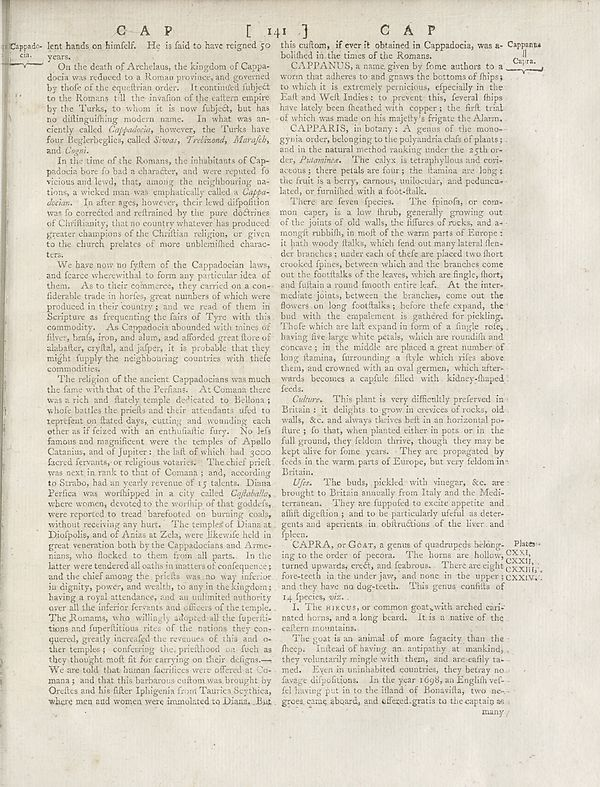
\includegraphics[width=0.85\textwidth]{../scans/page-1670-ced69857efba.jpg}
\caption*{Source scan: \texttt{page-1670-ced69857efba.jpg}}
\end{figure}

\end{document}
